\begin{figure}
	\centering
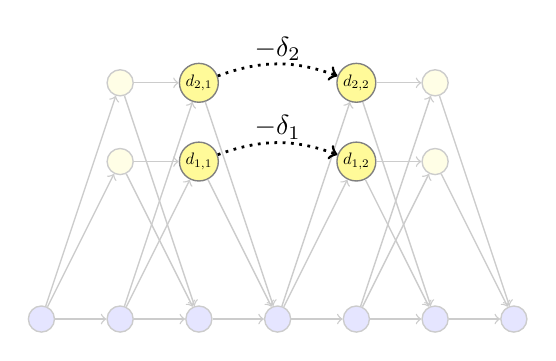
\begin{tikzpicture}
	\node[circle, fill=blue!10, line width=0.5pt, draw=black!20, minimum size=0.1in](one) at (0,0){};
	\node[circle, fill=blue!10, line width=0.5pt, draw=black!20, minimum size=0.1in](two) at (1,0){}; 
	\node[circle, fill=blue!10, line width=0.5pt, draw=black!20, minimum size=0.1in](three) at (2,0){};
	\node[circle, fill=blue!10, line width=0.5pt, draw=black!20, minimum size=0.1in](four) at (3,0){};
	\node[circle, fill=blue!10, line width=0.5pt, draw=black!20, minimum size=0.1in](five) at (4,0){};
	\node[circle, fill=blue!10, line width=0.5pt, draw=black!20, minimum size=0.1in](six) at (5,0){};
	\node[circle, fill=blue!10, line width=0.5pt, draw=black!20, minimum size=0.1in](seven) at (6,0){};
	
	\node[circle, fill=yellow!10, line width=0.5pt, draw=black!20, minimum size=0.1in](eight) at (1,2){};
	\node[circle, fill=yellow!40, line width=0.5pt, draw=black!50, minimum size=0.1in, inner sep=1pt](nine) at (2,2){\scalebox{0.6}{$d_{1,1}$}};
	\node[circle, fill=yellow!40, line width=0.5pt, draw=black!50, minimum size=0.1in, inner sep=1pt](ten) at (4,2){\scalebox{0.6}{$d_{1,2}$}};
	\node[circle, fill=yellow!10, line width=0.5pt, draw=black!20, minimum size=0.1in](eleven) at (5,2){};

	\node[circle, fill=yellow!10, line width=0.5pt, draw=black!20, minimum size=0.1in](twelve) at (1,3){};
	\node[circle, fill=yellow!40, line width=0.5pt, draw=black!50, minimum size=0.1in, inner sep=1pt](thirteen) at (2,3){\scalebox{0.6}{$d_{2,1}$}};
	\node[circle, fill=yellow!40, line width=0.5pt, draw=black!50, minimum size=0.1in, inner sep=1pt](fourteen) at (4,3){\scalebox{0.6}{$d_{2,2}$}};
	\node[circle, fill=yellow!10, line width=0.5pt, draw=black!20, minimum size=0.1in](fifteen) at (5,3){};

	\draw [->, line width=0.5pt, color=black!20] (one) -- (two);
	\draw [->, line width=0.5pt, color=black!20] (two) -- (three);
	\draw [->, line width=0.5pt, color=black!20] (three) -- (four);
	\draw [->, line width=0.5pt, color=black!20] (four) -- (five);
	\draw [->, line width=0.5pt, color=black!20] (five) -- (six);
	\draw [->, line width=0.5pt, color=black!20] (six) -- (seven);

	\draw [->, line width=0.5pt, color=black!20] (one) -- (eight);
	\draw [->, line width=0.5pt, color=black!20] (two) -- (nine);
	\draw [->, line width=0.5pt, color=black!20] (four) -- (ten);
	\draw [->, line width=0.5pt, color=black!20] (five) -- (eleven);
	\draw [->, line width=0.5pt, color=black!20] (eight) -- (three);
	\draw [->, line width=0.5pt, color=black!20] (nine) -- (four);
	\draw [->, line width=0.5pt, color=black!20] (ten) -- (six);
	\draw [->, line width=0.5pt, color=black!20] (eleven) -- (seven);
	\draw [->, line width=0.5pt, color=black!20] (eight)-- (nine);
	\draw [->, line width=0.5pt, color=black!20] (ten)-- (eleven); 

	\draw [->, line width=0.5pt, color=black!20] (one) -- (twelve);
	\draw [->, line width=0.5pt, color=black!20] (two) -- (thirteen);
	\draw [->, line width=0.5pt, color=black!20] (four) -- (fourteen);
	\draw [->, line width=0.5pt, color=black!20] (five) -- (fifteen);
	\draw [->, line width=0.5pt, color=black!20] (twelve) -- (three);
	\draw [->, line width=0.5pt, color=black!20] (thirteen) -- (four);
	\draw [->, line width=0.5pt, color=black!20] (fourteen) -- (six);
	\draw [->, line width=0.5pt, color=black!20] (fifteen) -- (seven);
	\draw [->, line width=0.5pt, color=black!20] (twelve)-- (thirteen);
	\draw [->, line width=0.5pt, color=black!20] (fourteen) -- (fifteen);
	\draw [dotted, color=black,-,line width=1pt] (nine) edge[->,bend left=20pt]node[above=-2.5pt]{\scalebox{1}{$-\delta_1$}}(ten); 
	\draw [dotted, color=black,-,line width=1pt] (thirteen) edge[->,bend left=20pt]node[above=-2.5pt]{\scalebox{1}{$-\delta_2$}}(fourteen); 

\end{tikzpicture}
	\caption{Relationship between exit nodes (left) and entrance nodes (right) as $\delta$}
	\label{fig:graphDelta}
\end{figure} 
